\documentclass{article}

\usepackage[spanish]{babel}
\usepackage[numbers,sort&compress]{natbib}
\usepackage{graphicx}
\usepackage{url}
\usepackage{amsmath}
\usepackage{hyperref}
\usepackage[top=30mm, bottom=40mm, left=15mm, right=15mm]{geometry}
\usepackage{listings}
\usepackage{subfig}
\usepackage{color}
\usepackage{multirow}

\setlength{\parskip}{2mm}
\setlength{\parindent}{0pt}
\definecolor{dkgreen}{rgb}{0,0.6,0}
\definecolor{gray}{rgb}{0.3,0.3,0.3}
\definecolor{orange}{rgb}{0.8,0.4,0}
\definecolor{mostaza}{rgb}{0.9,0.8,0.1}

\lstset{ %
  language=R,                     % the language of the code
  basicstyle=\footnotesize,       % the size of the fonts that are used for the code
  numbers=left,                   % where to put the line-numbers
  numberstyle=\tiny\color{gray},  % the style that is used for the line-numbers
  stepnumber=1,                   % the step between two line-numbers. If it's 1, each line
                                  % will be numbered
  numbersep=5pt,                  % how far the line-numbers are from the code
  backgroundcolor=\color{white},  % choose the background color. You must add \usepackage{color}
  showspaces=false,               % show spaces adding particular underscores
  showstringspaces=false,         % underline spaces within strings
  showtabs=false,                 % show tabs within strings adding particular underscores
  frame=single,                   % adds a frame around the code
  rulecolor=\color{black},        % if not set, the frame-color may be changed on line-breaks within not-black text (e.g. commens (green here))
  tabsize=2,                      % sets default tabsize to 2 spaces
  captionpos=b,                   % sets the caption-position to bottom
  breaklines=true,                % sets automatic line breaking
  breakatwhitespace=false,        % sets if automatic breaks should only happen at whitespace
  title=\lstname,                 % show the filename of files included with \lstinputlisting;
                                  % also try caption instead of title
  keywordstyle=\color{orange},      % keyword style
  commentstyle=\color{dkgreen},   % comment style
  stringstyle=\color{mostaza},      % string literal style
  escapeinside={\%*}{*)},         % if you want to add a comment within your code
  morekeywords={*,...}            % if you want to add more keywords to the set
} 

\author{Marco Antonio Guajardo Vigil  2095}
\title{\textbf{Pr\'actica 5: Método Monte-Carlo} \\ Simulaci\'on de sistemas}
\date{26 de febrero, 2019}

\begin{document}

\maketitle

\section{Introducci\'on}
El m\'etodo Monte-Carlo es id\'oneo para situaciones en las cuales alg\'un valor o alguna distribuci\'on no se conoce y resulta complicado de determinar de manera anal\'itica \cite{SatuP5}.
Para esta pr\'actica se ocupa estimar el valor de la integral $f(x)$ \eqref{fx}, cuyo valor dado en siete cifras es de \textbf{0.0488341}, obtenido de \textit{Wolfram Alpha} \cite{WA}.

\begin{equation}
f(x) = \int_{3}^{7}\frac{1}{exp(x) + exp(-x)} dx
\label{fx}
\end{equation}

La figura \ref{fig:fx} muestra la forma que tiene la funci\'on $f(x)$.

Se utiliza la funci\'on $g(x) = \frac{2f(x)}{\pi}$ para as\'i obtener una distribuci\'on v\'alida, ya que,

\begin{equation}
\int_{-\infty}^{\infty}\frac{2}{\pi}f(x) = 1
\end{equation}

Se crea un generador con la funci\'on $g(x)$ para crear valores que se normalizan para que el estimado sea de la funci\'on $f(x)$, la figura \ref{fig:gx} representa la funci\'on $g(x)$.

\section{Implementaci\'on de R}
Para la elaboraci\'on de este experimento, se hace uso de un software libre para computaci\'on estad\'istica y gr\'aficos llamado \citet{R}, el cual nos permite realizar los c\'alculos necesarios para dicho experimento. Con \'el, se pueden controlar los datos estad\'isticos que se ocupan para dar seguimiento con la pr\'actica, se necesita graficarlos para as\'i poder compararlos mejor, ya que se maneja una cantidad de datos considerable y trabajaremos con ellos en forma estad\'istica, por lo tanto, se recomienda el uso de este software ya que ayuda a paralelizar las acciones que sean necesarias, as\'i se ahorra tiempo, haci\'endolas simult\'aneamente.

\begin{figure}[h!]
\centering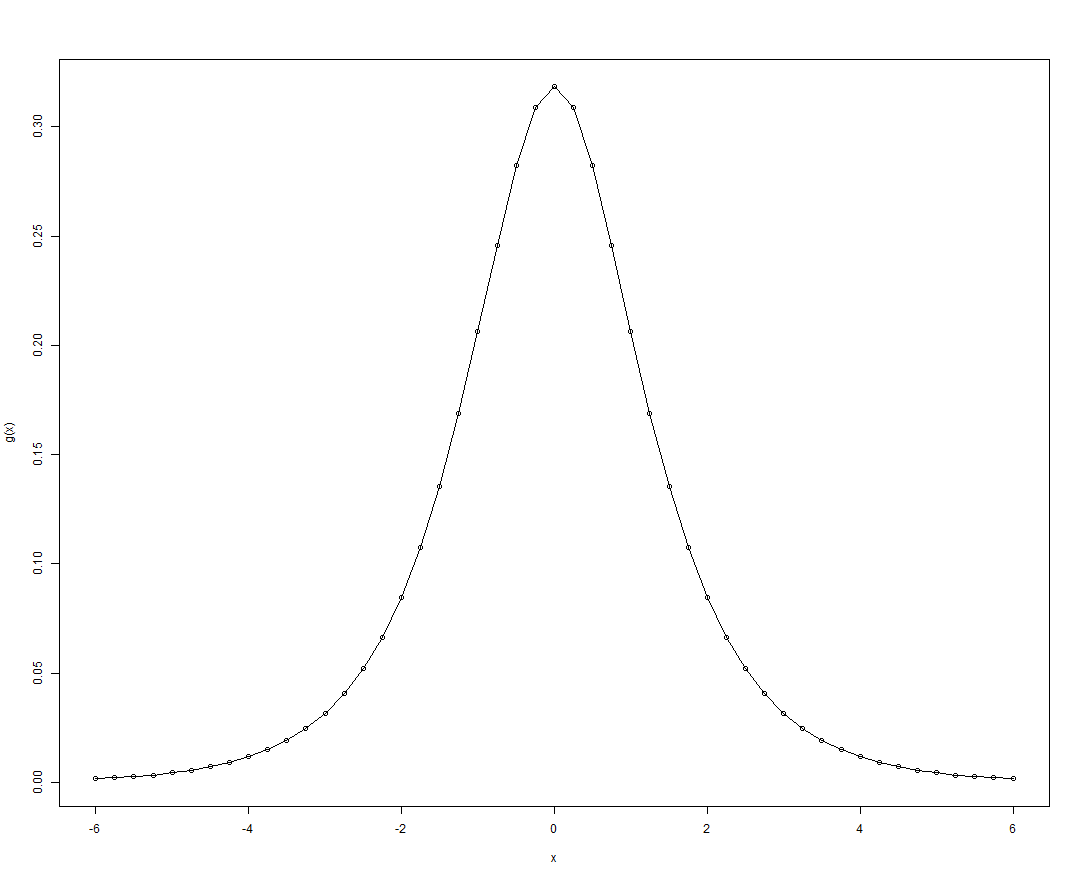
\includegraphics[width=110mm]{p5f.png}
\caption{Gr\'afica de la funci\'on $f(x)$}
\label{fig:fx}
\end{figure}

\begin{figure}[h!]
\centering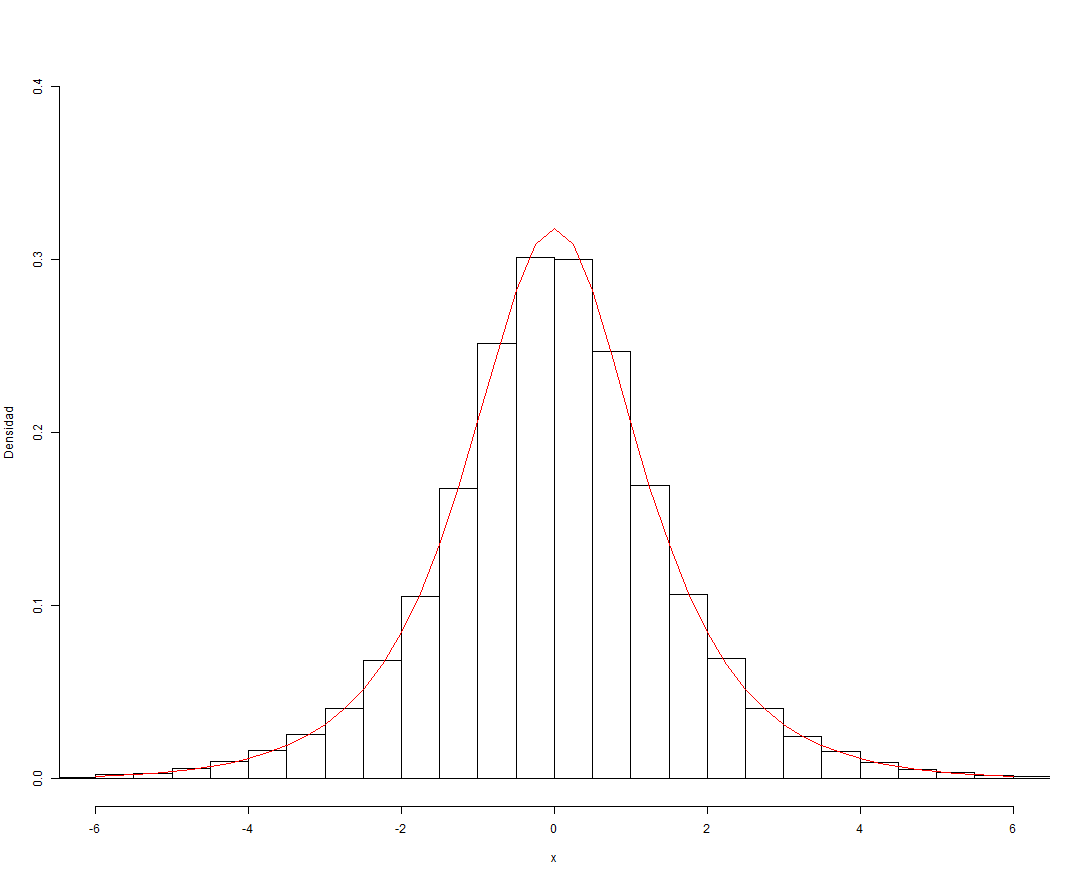
\includegraphics[width=110mm]{p5m.png}
\caption{Histograma de $g(x)$ comparado con $g(x)$.}
\label{fig:gx}
\end{figure}

\newpage

\section{Experimentaci\'on}

Para la elaboraci\'on de este experimento, se hace uso de un paquete de R llamado \textit{distr}.
Se crea un data.frame() llamado \textbf{datos} (en el cual se almacenan los valores de las r\'eplicas, muestras y resultados) y otro llamado \textbf{decimas} para comparar cuantas d\'ecimas se aproxim\'o con tal muestra.

\begin{lstlisting}[language=R]
datos <- data.frame()
cuantos <- 500 #Cuantos valores se manejan
replicas <- 30
pedazos <- c(500,1000,1500,2000,5000,10000)
valor <- 0.0488341
decimas <- data.frame()
lista <- NULL
\end{lstlisting}

Donde \textbf{pedazos}, l\'inea 4 del c\'odigo, refiere al n\'umero de muestras que se usan para el acercamiento al valor estimado de la integral.

Para controlar el manejo de las muestras a usar y el n\'umero de r\'eplicas que tiene cada muestra se utiliza el c\'odigo:

\begin{lstlisting}[language=R]
for (pedazo in pedazos) {
  for (rep in 1:replicas) {
    montecarlo <- foreach(i = 1:cuantos, .combine=c) %dopar% parte()
    integral <- sum(montecarlo) / (cuantos * pedazo)
    resultado <- (pi / 2) * integral
    lista <- c(lista, resultado)
    error <- valor - resultado
    resultados <- c(rep, pedazo, valor, resultado, error)
    datos <- rbind(datos, resultados)
  }
  print(length(lista))
  decimas <- rbind(decimas, c(min(lista), max(lista), pedazo))
  lista <- NULL
}
stopCluster(cluster)
\end{lstlisting}

Se crea una gr\'afica que muestra el error que se presento relacionado con las muestras y otra para las estimaciones obtenidas con relaci\'on a las muestras.

\begin{lstlisting}[language=R]
png("error.png")
boxplot(data=datos, error~muestra, xlab="Tama\~o de muestra", ylab="Error", main="", col = "orange")
abline(h=0, col="red", pch=20)
graphics.off()

png("aproximacion.png")
boxplot(data=datos, resultado~muestra, xlab="Tama\~o de muestra", ylab="Resultados", main="", col = "blue")
abline(h=valor, col="red", pch=20)
graphics.off()
\end{lstlisting}

\newpage

\section{Resultados y concluciones}

\begin{figure}[h!]
\centering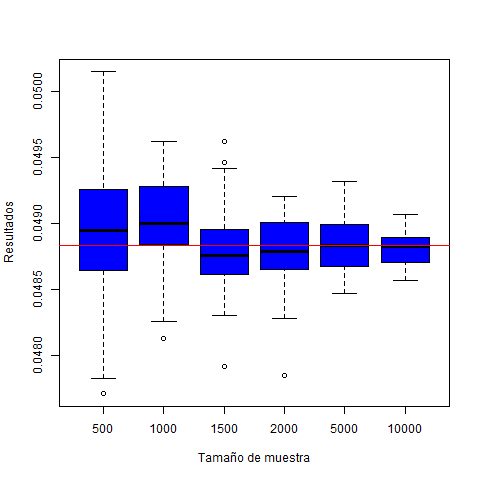
\includegraphics[width=120mm]{aproximacion.png}
\caption{Gr\'afica de estimaciones obtenidas con relaci\'on a las muestras.}
\label{fig:aprox}
\end{figure}

En la figura \ref{fig:aprox} se observa que en cuanto la muestra sea cada vez mayor a la anterior, esta da aproximaciones muy cercanas al valor de la integral $f(x)$, lo cual hace que el numero de decimas acertadas sean cada vez m\'as, esto debido a que se toma mayor muestra la cual aumenta la posibilidad de que los valores generados en esa muestra se encuentren debajo de la curva de la integral.
La l\'inea roja representa el valor de la integral \textbf{0.0488341}.

\newpage

\begin{figure}[h!]
\centering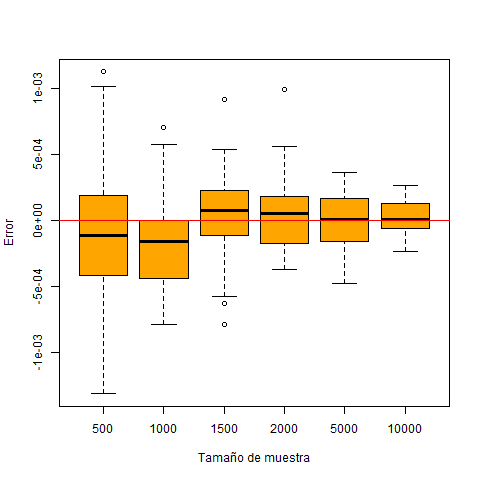
\includegraphics[width=100mm]{error.png}
\caption{Gr\'afica de errores con relaci\'on a las muestras.}
\label{fig:error}
\end{figure}

La figura \ref{fig:error} muestra el error de aproximaci\'on que tienen los resultados estimados con relaci\'on de las muestras, cada vez que aumenta la muestra el error se va haciendo menos notorio a comparaci\'on de una muestra peque\~na como lo es con \textbf{500}, la l\'inea roja representa el error al momento en el que este llega a ser nulo, tomando el valor de \textbf{0}.

A los valores obtenidos de cada muestra se obtuvo el m\'aximo y m\'inimo para asi poder observar mejor los valores estimados, como se muestra en el cuadro \ref{tabla:valores}.

\begin{table}[htb]
\centering
\begin{tabular}{|l|l|l|}
M\'inimo & M\'aximo & Muestra \\
\hline
0.04770823 & 0.05014610 & 500 \\ \hline
0.04812920 & 0.04961831 & 1000 \\ \hline
0.04791557 & 0.04962041 & 1500 \\ \hline
0.04784331 & 0.04920205 & 2000 \\ \hline
0.04846849 & 0.04931421 & 5000 \\ \hline
0.04856934 & 0.04906508 & 10000 \\ \hline
\end{tabular}
\caption{Valores estimados con relaci\'on a las muestras.}
\label{tabla:valores}
\end{table}

Para muestras de \textbf{1,000} la aproximaci\'on al valor es de 3 d\'ecimas, con \textbf{10,000} muestras empieza aproximar entre seis y siete d\'ecimas.

\newpage

\bibliographystyle{plainnat}
\bibliography{Bibliografias}
\end{document}